This chapter covers details of camera, the main sensor used in \acrshort{vo}. Different types of cameras, their advantages and drawbacks with important properties for \acrshort{vo} implementation, selected cameras and their calibrations are explained. 

\section{Classification of Camera}
Cameras can be classified mainly into two types :
\begin{enumerate}
	\item Passive Camera
	\begin{enumerate}
		\item Monocular
		\item Stereo
		\item Omnidirectional
	\end{enumerate}
	\item Active Camera
	\begin{enumerate}
		\item Time of flight (TOF)
		\item RGB-Depth
	\end{enumerate}
\end{enumerate}
Passive cameras are mostly used in \acrshort{vo} experiments. Some common types are shown in the figure \ref{fig:cameras}.
\begin{figure}[h]
	\centering
	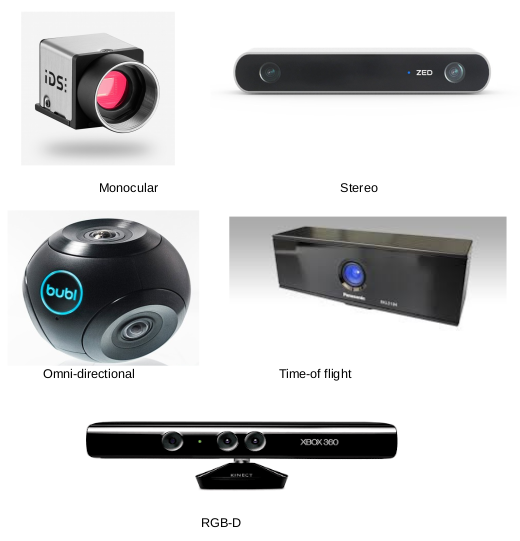
\includegraphics[width=1.0\textwidth]{cameras}
	\caption{Different types of cameras used in \acrshort{vo} \cite{ids},\cite{kinect},\cite{zed}, \cite{omni},\cite{tof}}
	\label{fig:cameras}
\end{figure}

\section{Important Properties}
There are some criteria to select proper camera model in order to achieve high accuracy and robustness. First important property is shutter technology. Rolling shutter cameras may consist geometric distortions in the image during camera motion or in dynamic scene conditions. It reduces accuracy especially in direct \acrshort{vo} methods. As discussed in section \ref{direct} direct methods do not optimize geometric noise. Another important property is Field of view (FOV) of a camera. Large \acrshort{fov} cameras would have enough information (features) to track camera motion which helps to increase robustness during pure rotations. Higher camera resolution can increase the accuracy of 3D pose estimation of the features but at the same time it will increase the computation costs due to more memory usage. Auto-exposure may reduce the accuracy of direct \acrshort{vo} methods. Therefore, it is important to use fixed-focus camera for the direct approaches. Finally, suitable lens size can reduce the effect of vignetting which is defined as radial falloff of intensity from the image center \cite{vignette}. It occurs due to blockage of light due to some camera parts or hoods attached to lens.

\section{Camera Selection}
Monocular cameras are consist of one image sensor and lens. Depending on types of lens they can be modeled as pinhole, fish-eye (wide \acrshort{fov}) or omnidirectional \cite{multiview_geometry}. The main disadvantage of monocular camera is that they can not estimate the true depth of the scene. Absolute scale can be estimated with using some prior knowledge like known object-size \cite{citymodel}, deep learning methods as explained in \cite{synthetic}, \cite{deepl} or geometric constraints like known camera heights for planer camera motion as described in \cite{ground}, \cite{geometric} and \cite{planer} or fusion with some extra sensor like \acrshort{imu}, \acrshort{gps}, 2D \acrshort{lidar} etc. \\
\newline
Stereo cameras are consist of two image sensors inspired from humans with fixed distance (baseline) between them. Both sensors are synchronized to capture images at the same time. Stereo camera can sense the depth of world by finding correspondences in the left and right image taken at same time. The accuracy of depth estimation depends on the baseline. When depth increases with fixed baseline, it can be gradually degraded to monocular case. Stereo camera required good calibration, stereo rectification and undistortion. \\
\newline
A combination of both the types discussed above is called as RGB-D camera. It consists of a depth sensor in addition to monocular camera based on time of flight. For every pixel depth can be measured and register into depth map for every image with no need of stereo. Limitation of RGB-D is that they can be either used for indoor application or up to some limit of depth. The table \ref{table:cameracomp} shows some advantages and disadvantages of these cameras.\\
\begin{table}[h!]
	\centering
	\begin{tabular}[c]{ |m{0.12\linewidth} | m{0.40\linewidth} | m{0.40\linewidth} |}
		\hline 
		\textbf{Camera} & \textbf{Advantages}  & \textbf{Disadvantages} \\ [1ex] \hline
		Monocular & \begin{itemize} 
				 		\item Cheaper, light weight
						\item Small size, low computational cost 
						\item Simple calibration 
				   \end{itemize} & 
			       \begin{itemize} 
			       	\item Suffers from scale ambiguity
			       	\item \acrshort{vo} fails in pure rotations
			       	\item Slow \acrshort{vo} initialization
			       \end{itemize} \\ \hline
		Stereo & \begin{itemize} 
					\item 3D vision from one stereo pair
					\item Easy \acrshort{vo} initialization
				\end{itemize} & 
				\begin{itemize} 
					\item Expensive and complex calibration
					\item High processing time and cost
					\item Complex synchronization
				\end{itemize} \\ \hline
		RGB-D  & \begin{itemize} 
					\item Provides depth map 
					\item Easy \acrshort{vo} initialization
				\end{itemize} & 
				\begin{itemize} 
					\item Limited to indoor and small depth environment
					\item High power consumption
					\item Complex calibration
				\end{itemize} \\ \hline
	\end{tabular}
	\caption{Advantages and disadvantages of cameras used in \acrshort{vo}}
	\label{table:cameracomp}  
\end{table}
\newline
Based on discussion of camera properties above monocular camera are selected due to their simplicity. The two different types of monocular cameras are selected based on availability namely SICK-Picocam of model number -I2D304C-RCA11 and a rolling shutter Genius widecam (F100)
(figure \ref{fig:cameras_used}) in order to compare the different technology. Best performing camera will be selected for the adaptation and further research. Table \ref{table:camera_prop} illustrate the properties of these cameras in comparison with IDS UI-3241LE which is used in TUM- benchmark dataset \cite{photometrically}.
\begin{figure}[h!]
	\begin{subfigure}{.5\textwidth}
		\centering
		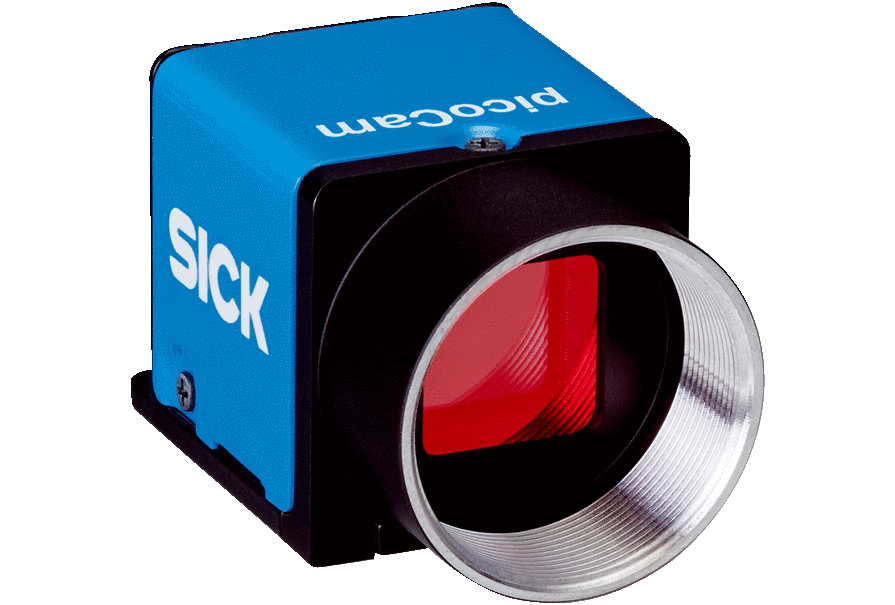
\includegraphics[width=1.0\linewidth]{picocam}
		\caption{Picocam-I2D304C-RCA11 \cite{picocam}}
		\label{fig:picocam}
	\end{subfigure}%
	\begin{subfigure}{.5\textwidth}
		\centering
		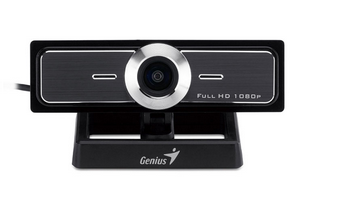
\includegraphics[width=1.0\linewidth]{genius}
		\caption{ Genius widecam (F100) \cite{genius}}
		\label{fig:webcam}
	\end{subfigure}
	\caption{Two cameras used for \acrshort{vo} experiments}
	\label{fig:cameras_used}
\end{figure}

\begin{table}[h!]
	\centering
	\begin{tabular}{ | l | l | l | l |}
		\hline
		\textbf{Model} & \textbf{SICK Picocam}  & \textbf{Genius widecam}  & \textbf{IDS UI-3241LE}  \\  
		              & \textbf{I2D304C-RCA11} & \textbf{F100} &  \\  
		\hline
		Shutter technology & Global & Rolling shutter & Global and Rolling \\ 
		\hline
		Lens type         & C-mount & attached        & S-mount \\ 
		\hline
		FPS               & 19      & 30              & 60\\ 
		\hline
		Resolution       & 2048*2048  &  1280 * 720   & 1280 *1024 \\
		 \hline
		Exposure time (ms) & 0.0009 - 2000 & auto &    \\
		 \hline
		Sensor size (mm) & 11.26 x 11.26 & 6.784 x 5.427 &  \\
		 \hline
		FOV (degree) &  90(diag) &  120 & 98 x 79  \\
		 \hline
		Lens &  Kowa   &   & Lensagon \\
		     &  LM8HC  &   & BM4018S118  \\
		 \hline
	\end{tabular}
    \caption{Comparison of properties of cameras used in this thesis with IDS UI-324LE used in TUM-benchmark dataset}
    \label{table:camera_prop}
\end{table}
\section{Camera Calibration}
For any \acrshort{vo} method camera calibration is an important part. Though some cameras are manufactured very well, they still have some distortions. Using cameras directly without calibration may lead to wrong trajectory estimation and \acrshort{vo} may not perform well. Camera calibration can be classified into two types namely Geometric and Photometric. Geometric calibration covers intrinsic and distortion parameters. While photometric focuses on the effect of shutter speed, motion blur and vignette. It is mostly recommended for cameras which have rolling shutter and auto-exposure technology. Moreover, It is also recommended for direct approaches which tracks image pixel intensity values for motion estimation \cite{yang2018challenges}. This section will discuss only geometric calibration. Photometric calibration is not in the scope of this thesis because of its complexity and non-necessity for any \acrshort{vo} method. The more details about photometric calibration and its effects can be found in \cite{yang2018challenges} ,\cite{photometrically}, \cite{bergmann2017online} and \cite{vignette}.\\

\subsection{Pinhole Camera Model}
Monocular camera with normal lens can be simply modeled as pinhole camera model as shown in figure \ref{fig:pinhole}. A 2D image point  $ m = [u,v]^{T} $ on image with corresponding 3D point $ M = [ X,Y Z]^{T} $ in world can be formed by an optical ray from M passing through camera optical center C by intersecting image plane at m. The relation between M and m in homogeneous coordinates can be given by: 
\begin{equation*}
sm= KTM 
\end{equation*} 
with
\begin{equation*}
K = \begin{bmatrix}
f_{x} & \gamma & u_{o} \\
0    &  f_{y} & v_{o} \\
0    &   0    & 1 \\
\end{bmatrix}
\end{equation*} 
and
\begin{equation*}
T = \begin{bmatrix}
r_{11} & r_{12} & r_{13} & t_{1} \\
r_{21} & r_{22} & r_{23} & t_{2} \\
r_{31} & r_{32} & r_{33} & t_{3} \\
\end{bmatrix}
\end{equation*} 
s is scale factor. K is known as camera intrinsic matrix with $ (u_{0},v_{0}) $ being a principal point, $ (f_{x},f_{y}) $ being the focal length in pixels in x and y direction and $ \gamma $ is the skew between both image axis. T is the 3x4 transformation matrix with R and t being rotation and translation from world to camera frame also known as extrinsic parameters.\\
\begin{figure}[h!]
	\centering
	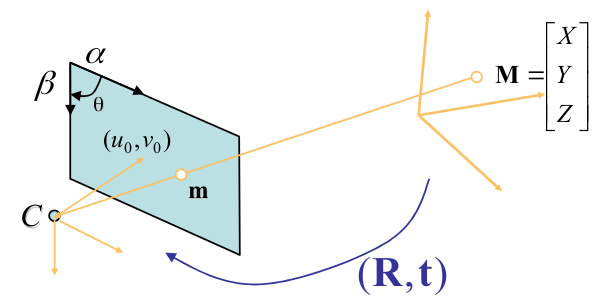
\includegraphics[width=1.0\textwidth]{pinhole}
	\caption{Pinhole camera model. C is camera center, m is 2D image point corresponding to 3D object point M, R and t are rotation and translation resp \cite{cameracalib}.}
	\label{fig:pinhole}
\end{figure}
\newline
The purpose of camera calibration is to compute these parameters known as intrinsic and extrinsic parameters. The combination of K and T is also known as projection matrix denoted by $ P = K \begin{bmatrix} 
            R & t \\
            \end{bmatrix} $.
There are total 11 parameters to be determine of which 6 are degrees of freedom and 5 are intrinsic parameters $ (f_{x},f_{y},u_{0},v_{0}, \gamma) $. There exists many techniques of geometric calibration based on type of the reference objects. They can be found in \cite{cameracalib}. In this thesis 2D plane based technique \cite{zhangcalib}, \cite{sturmcalib} is used due to its simplicity and good accuracy. The mathematical derivation can be found in \cite{cameracalib}.\\
\newline
Camera lens may also consists distortion. There are two types of distortion can be found in pinhole camera lens namely radial and tangential distortion. As shown in figure \ref{fig:distortion} radial distortion generates due to distortion of optical rays at lens edge which depends on the size of lens. i.e. smaller lens consist higher radial distortion. The relation between distorted and undistorted pixels coordinates can be estimated as:
\begin{equation*}
p_{undistorted} = p_{distorted} /(1+ k_{1}r^{2}+k_{2}r^{4}+k_{3}r^{6})
\end{equation*} 
where $ k_{1},k_{2},k_{3} $ are known as radial distortion coefficients.\\
\newline
Tangential distortion generally occurs due to non-parallel lens and sensor. It depends on mounting and manufacturing of camera. There are only two coefficients which needs to corrected known as $p_{1} $ and $ p_{2} $. In simple camera calibration there are five distortion parameters and 5 intrinsic parameters needs to be estimated. There are some open-source software tools are already available with code. such as Matlab, OpenCV etc. OpenCV camera calibration module has been used in this scope \cite{opencvcalib}. 
\begin{figure}[h!]
	\centering
	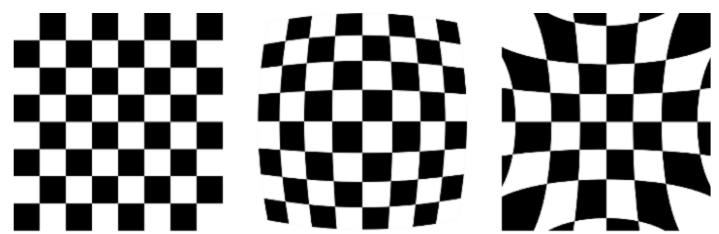
\includegraphics[width=1.0\textwidth]{distortion}
	\caption{Radial distortion created by camera lens \cite{opencvcalib}}
	\label{fig:distortion}
\end{figure}

\subsection{Calibration Procedure}
This section covers the calibration procedure in brief. Different types of calibration patterns can be used such as chessboard, AR tags, data matrix, symmetric and asymmetric circular grid as shown in figure \ref{fig:pattern}. In this thesis work a symmetric circular grid pattern is used for picocam and chessboard pattern is used for genius widecam. The size of circular pattern is relatively larger than that of chessboard due to higher resolution of picocam.\\
\begin{figure}[h!]
	\centering
	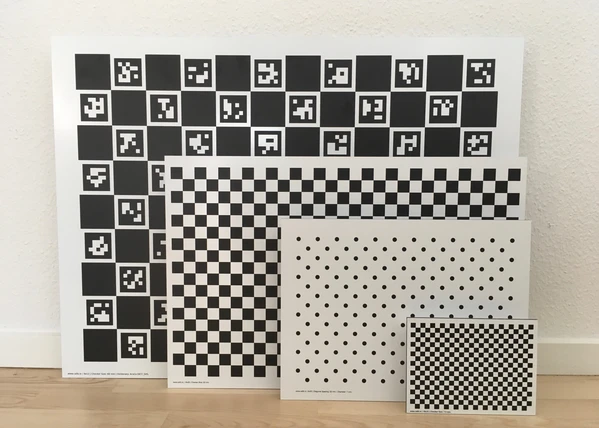
\includegraphics[width=1.0\textwidth]{pattern}
	\caption{Types of calibration pattern used for camera calibration. such as AR tags, chessboard, circles grid \cite{calibio}}
	\label{fig:pattern}
\end{figure}
\newline
The general steps are as follows \cite{cameracalib}:
\begin{enumerate}
	\item Print the target pattern with sufficient size and fix it to planar surface.
	\item Grab some images of the pattern in different orientation and positions by moving either the target or camera.
	\item Detect the all corners or features of the pattern in all images.
	\item Compute the intrinsic and extrinsic parameters.
	\item Estimate the distortion coefficient.
	\item Refine all parameters and project the 3D object points using computed parameters.
	\item Compute the reprojection error, accept the result if error is with in limit otherwise repeat the procedure by taking more number of images until error is in limit.
\end{enumerate}

\subsection{Recommendations for good calibration}
Accurate intrinsic calibration is one of the most important factor for \acrshort{vo} algorithms regardless of its approach. This section describes some of the best practices to achieve higher accuracy. They are:
\begin{enumerate}
	\item Target pattern should be of right size. Optimal should be nearly half of the total area seen in front of camera. Calibration accuracy also depends on target print quality.
	\item Camera and lens should be focused on target. The setting should remains unchanged during \acrshort{vo} experiment also. 
	\item Images should be collected from different positions and in all orientations. It is recommended for good estimation of lens distortion and camera focal length.
	\item The surrounding area should have constant and rather diffused lighting. 
	\item The number of images should be enough including all possible camera poses.
	\item Either target or camera should be mount rigidly during whole process. Camera should not move while image capturing.
	\item If there is any bad images which consist higher reprojection error then it should be removed.
	\item Lower reprojection error doesn't mean that the camera calibration is accurate. It might be case of overfitting. Every reprojection error should be analyse and images with higher error should be removed and recalibration should be done until satisfactory results has arrived.
\end{enumerate}

\subsection{Calibration result}
As discussed two cameras are selected in this scope of work. First picocam is calibrated using chessboard as shown in figure \ref{fig:chessboard} but the results found not accurate which lead to bigger calibration target which is circular grid pattern. Picocam is calibrated using symmetric circular grid as shown in figure \ref{fig:circular_grid}. While Genius widecam is calibrated with help of 8 x 8 size chessboard as shown in figure \ref{fig:chessboard}. More than 150 images were taken for both cameras. Resolution for Picocam is 1024 x 1024 and for Genius Widecam it is 1080 x 720 pixels. Calibration results for both cameras can be found in \ref{section:A.2}. Figure \ref{fig:pattern_view} shows Picocam poses taken in all possible locations with respect to the pattern. Average reprojection error estimated for picocam is below 0.010 pixels which can be seen in figure \ref{fig:reproj}.\\
\begin{figure}[h!]
	\begin{subfigure}{0.5\textwidth}
		\centering
		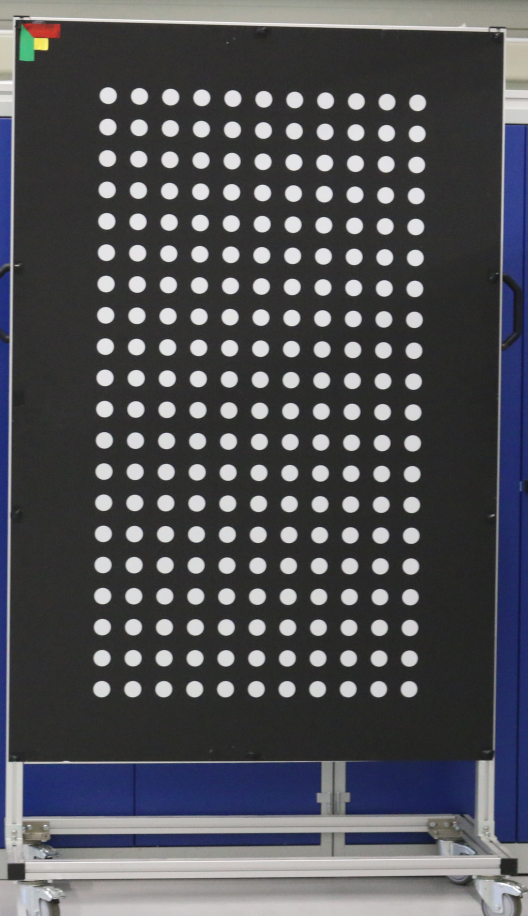
\includegraphics[width=1.0\textwidth]{circular_grid}
		\caption{Symmetric circular pattern used for Picocam}
		\label{fig:circular_grid}
	\end{subfigure}%
	\begin{subfigure}{0.5\textwidth}
		\centering
		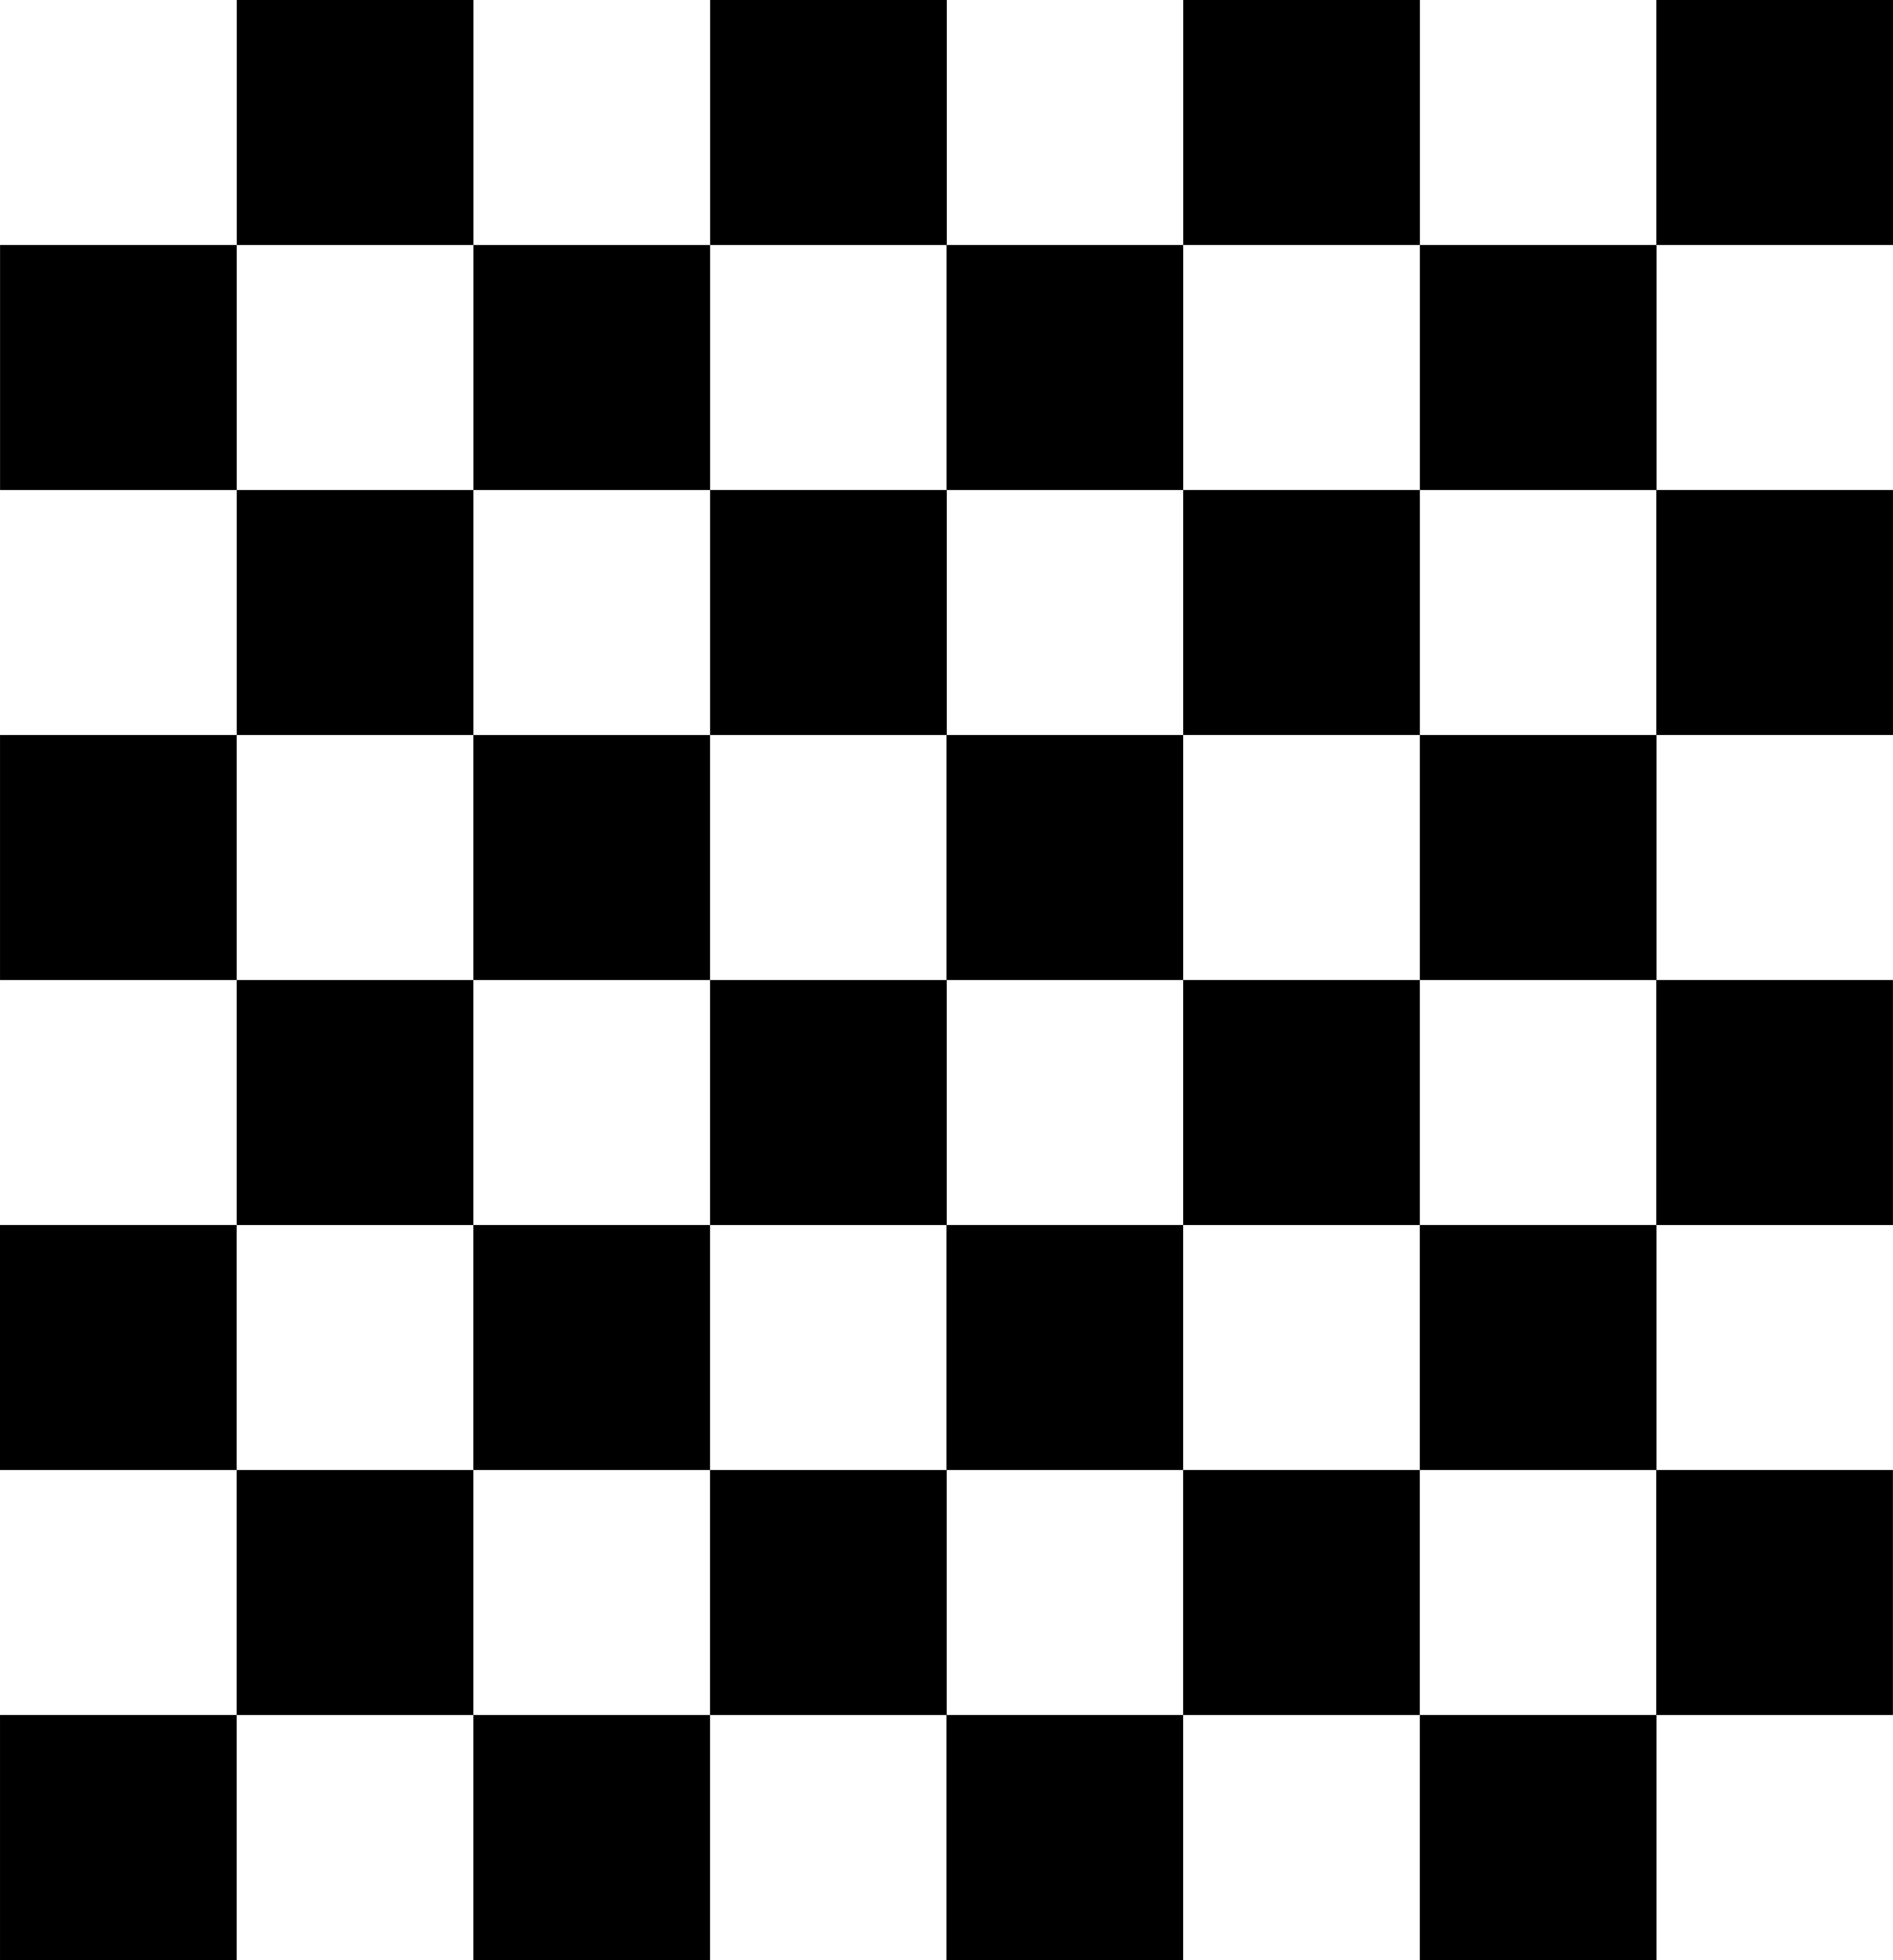
\includegraphics[width=0.7\textwidth]{chessboard}
		\caption{Chessboard pattern of size 8 x 8 used for Genius Widecam}
		\label{fig:chessboard}
	\end{subfigure}
	\caption{Different patterns used for camera calibration}
	\label{fig:patterns}
\end{figure}
\begin{figure}[h!]
	\centering
	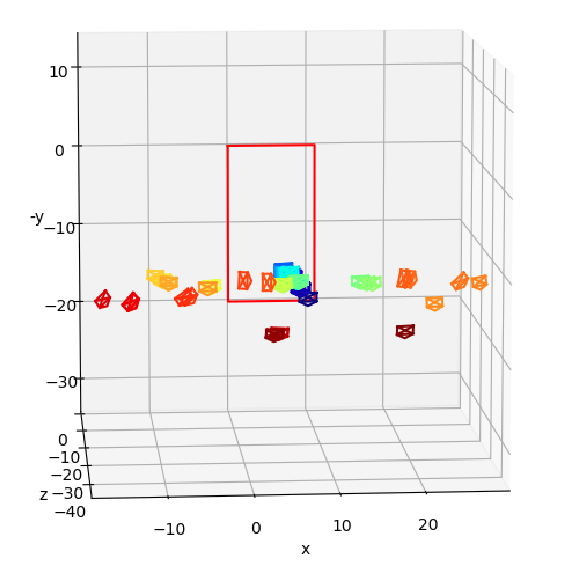
\includegraphics[width=1.0\textwidth]{pattern_view}
	\caption{Pattern centric view with rectangle as pattern and pentagons as camera}
	\label{fig:pattern_view}
\end{figure}
\begin{figure}[h!]
	\centering
	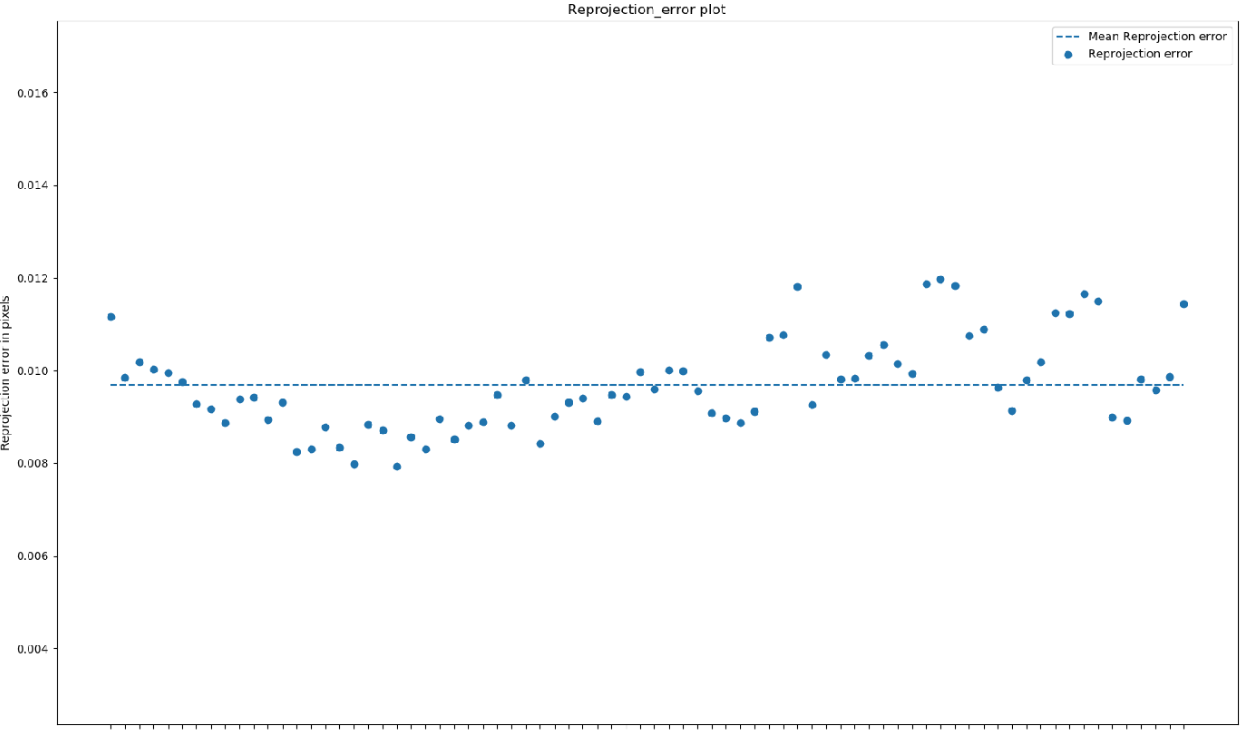
\includegraphics[width=1.0\textwidth]{reproj_error}
	\caption{Reprojection error plot for Picocam}
	\label{fig:reproj}
\end{figure}